\clearpage
%//==============================--@--==============================//%
\subsection{P5 | Espaçamento variável entre as tomas de medicamento}
\label{subsec:P5}
O espaçamento variável depende do objetivo do modelo de tratamento proposto, nomeadamente, \textbf{erradicação} ou \textbf{supressão} do tumor:
%//==============================--I--==============================//%
\vspace{-1em}
\subsubsection{$\pmb{\xrightarrow[]{}}$ \textit{Front-Load dosing}}
\label{subsubsec:front-load-dosing}
\vspace{-2.5em}
\hspace*{-0cm}\begin{wrapfigure}[11]{l}{0.5\textwidth}
    \centering
    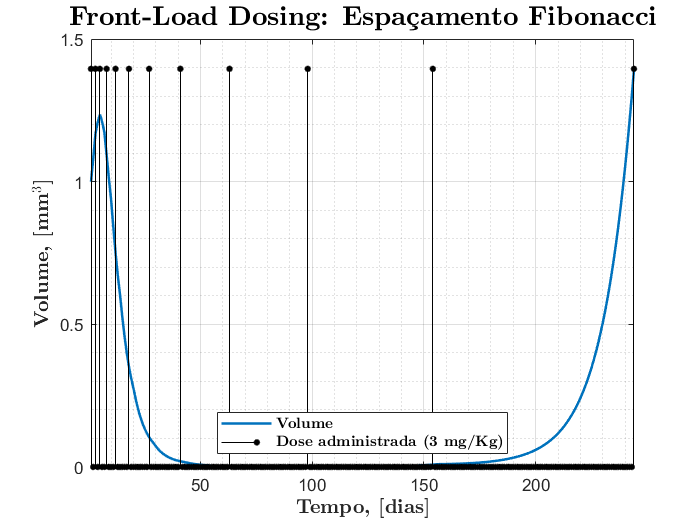
\includegraphics[width=0.5\textwidth]{img/perguntas/P5/P5-Fib.png}
    \vspace{-0.1em}\begin{minipage}{1\linewidth}
        \caption{Simulação da administração \textit{Front-Load} mediante a sequência de Fibonacci.}
        \label{fig:P5-fib}
    \end{minipage}
\end{wrapfigure}

\begin{quote}
     \textit{``Dosing by ``front-loading'' has thus become the mainstay of treatment, owing largely to theoretical and laboratory studies over the past 40 years (...)''}\cite{Hahnfeldt2003-oy}
\end{quote}

\textbf{Front-Loading} $\rightarrow$ Administração de doses elevadas de fármaco mediante espaçamentos de curta duração na fase inicial de terapia.

\vphantom{esperiencia123}

\vphantom{esperiencia123}

\vphantom{esperiencia123}

A administração \textit{Front-Load} procura \underline{erradicar} o tumor nos estágios iniciais de desenvolvimento, evitando aquisições elevadas de resistência (vide \hyperref[subsec:P6]{secção P6}). A simulação evidencia uma rápida diminuição do volume cancerígeno com aproximação do limite assíntótico em $V = 0$ na marca dos 50 dias e ainda um baixo crescimento máximo de 23\% do volume inicial (5º. dia). 

Em contexto real, esta impressionante diminuição de volume\footnotemark[7] revela-se inconsistente: a remissão é muitas vezes seguida de reincidência (de forma análoga ao crescimento na marca dos 150 dias, na \hyperref[fig:P5-fib]{Fig. 9})\footnotemark[8]. Esta administração apresenta alguns pontos pouco favoráveis:
\vspace{-0.75em}
\begin{enumerate}
    \itemsep 0em 
    \item Aplicação de uma elevada dose de fármaco num curto espaço de tempo leva a um incremento da carga tóxica no corpo hospedeiro (vide \hyperref[subsec:P2]{secção P2}).
    \vspace{-0.5em}\item Dificuldade em limitar a ação do fármaco ao tumor: \textit{``threat to the bone marrow and other at-risk stem cell compartments.''}\cite{Hahnfeldt2003-oy}
    \vspace{-0.5em}\item Eficácia reduzida em massas cancerígenas heterogéneas (\textit{``The cell population subject to treatment is in general not uniform, consisting instead of sensitive and resistant subpopulations.''})
\end{enumerate}

%//==============================--II-==============================//%
\vspace{-2em}
\subsubsection{$\pmb{\xrightarrow[]{}}$ \textit{Metronomic dosing}}
\label{subsubsec:metronomic-dosing}
\begin{quote}
    ``\textit{Recently, a revolutionary form of chemotherapy has emerged. Metronomic chemotherapy (...)}''\cite{elisa_2017}
\end{quote}
A administração metronómica depende de uma administração continua e periódica de baixa dosagem (\textit{minimum biologically effective dose}\cite{elisa_2017}) e consequentemente de baixa toxicidade, sem períodos de pausa entre fases de administração (\textit{no prolonged drug-free breaks}\cite{elisa_2017}). Esta administração não procura erradicar mas sim \underline{suprimir} o tumor: \textit{``Patient survival is not incompatible with tumor presence.''}\cite{Hahnfeldt2003-oy}.

Este modelo de espaçamento preenche as lacunas do anterior:

\vphantom{esperiencia123}
\begin{enumerate}
    \itemsep 0em 
    \vspace{0em}\item Aplicação de baixas doses de fármaco, que por consequência, não excedem a dose permissível deste no organismo (\hyperref[subsec:P2]{secção P2}).
    \vspace{-0.5em}\item  Permite a restauração de células essenciais (\textit{``stemcell recovery''}\cite{Hahnfeldt2003-oy}).
    \vspace{-0.5em}\item  Limita a proliferação de células resistentes através da manutenção de uma elevada proporção de células sensíveis no seio do tumor: \textit{``due to competition for space and resources between these populations (...)''}\cite{elisa_2017}  $\xrightarrow[]{}$ \textit{Resensitization effect}\cite{Hahnfeldt2003-oy}.
\end{enumerate}

\vspace{-0.5em}
\noindent $\pmb{\star}$ \textbf{São considerados dois casos de espaçamento metronómico:}

%//==============================--II-==============================//%
\footnotetext[7]{Comparativamente à administração abordada \hyperref[subsubsec:P4a]{na secção 4 a)}}
\footnotetext[8]{Embora o recrescimento do tumor na simulação seja resultado da limitação da equação logística (vide \hyperref[subsubsec:P3c]{secção P3 c)}), podemos admitir esta reincidência perto da realidade.}
%//==============================--II-==============================//%
%\clearpage
%//==============================--i--==============================//%
\vspace{-1.5em}\paragraph{i) \textit{Pattern}}\mbox{}\\
\label{subsubsubsec:pattern}
\vspace{-2.5em}
\hspace*{-0cm}\begin{wrapfigure}[12]{l}{0.47\textwidth}
    \centering
    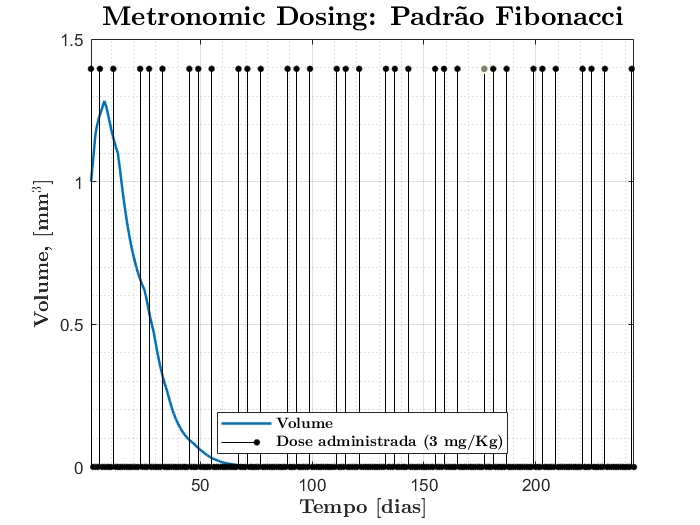
\includegraphics[width=0.5\textwidth]{img/perguntas/P5/P5-pattern.png}
    \begin{minipage}{2\linewidth}
        \caption{Sim. da administração mediante o 5º e 6º elemento da sequência, com \textit{rest period} = $10$d.}
        \label{fig:P5-pattern}
    \end{minipage}
\end{wrapfigure}

\vspace{-1.25em}
\begin{quote}
    \textit{``A general chemotherapeutic dosing regimen involves delivering a fixed pattern of equal doses, separated by ``rest periods'' \underline{to allow stemcell recovery}.''}\cite{Hahnfeldt2003-oy}
\end{quote}

A administração metronómica cíclica (\textit{metronomic pattern dosing}) evidencia uma regressão de volume tumoral menos célere que a observada no espaçamento \textit{Front-Load}, mantendo, no entanto, um baixo volume de forma contínua ao longo do tempo.

%//==============================--ii-==============================//%
%\vspace{-1.5em}
\paragraph{ii) \textit{Response to uneven vs. metronomic dosing}}\mbox{}\\
\vspace{-2em}
\label{subsubsubsec:amplitude-variation}
\begin{figure}[ht] 
    \begin{subfigure}[b]{0.5\linewidth}
        \centering
        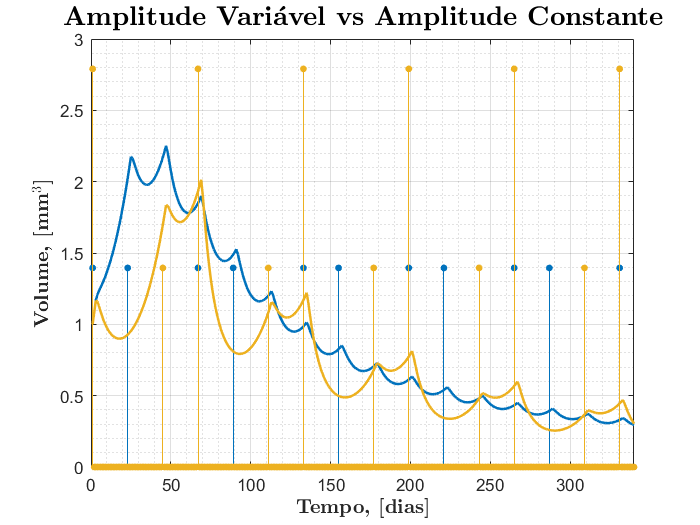
\includegraphics[width=0.8\linewidth]{img/perguntas/P5/P5-AmpVriation.png}
        \caption{Dose constante = 3 mg/kg a \textcolor{blue}{azul};\\ dose variável = 6 mg/kg, 0, 3 mg/kg periódicos a \textcolor{yellow}{amarelo}.} 
        \label{fig:AmpVarMatlab} 
        %\vspace{1ex}
    \end{subfigure}%% 
    \begin{subfigure}[b]{0.5\linewidth}
        \centering
        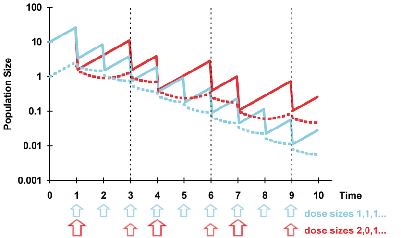
\includegraphics[width=0.8\linewidth]{img/perguntas/P5/P5-AmpVarDoc.png} 
        \caption{Dose constante = 1 mg/kg a \textcolor{blue}{azul};\\ dose variável = 2 mg/kg, 0, 1 mg/kg periódicos a \textcolor{red}{vermelho}.} 
        \label{fig:AmpVarDoc} 
        %\vspace{1ex}
    \end{subfigure}
    \vspace{-1.0em}\begin{minipage}{1\linewidth}
        \caption{Comparação entre espaçamentos constantes de dose variável e dose e permanente}
    \end{minipage}
\end{figure}

Tomando a abordagem metronómica como vetor de ataque preferível face à \hyperref[subsubsec:front-load-dosing]{\textit{Front-Load dosing}}, podemos ainda recorrer à comparação de uma administração equiespaçada no tempo de amplitude variável e metronómica de amplitude constante:
\vspace{-0.8em}
\begin{itemize}
    \item[$\rightarrow$] \textit{``Although the more up-front [amplitude variável] schedule is competitive early on, metronomic delivery provides better long-term suppression''}\cite{Hahnfeldt2003-oy} comprovada pela estabilidade da diminuição de volume \hyperref[fig:AmpVarDoc]{Fig. 11 (b)} a amplitudes constante e corroborada pela evolução observada na \hyperref[fig:AmpVarDoc]{Fig. 11 (a)}.
\end{itemize}

\noindent\textbf{Nota} $\rightarrow$ Vale salientar as regressões a pontilhado na \hyperref[fig:AmpVarDoc]{Fig. 11} representantes da evolução das células resistentes. É corroborado (através de simulações) o mencionado na \hyperref[subsubsec:metronomic-dosing]{secção anterior}: \textbf{o espaçamento metronómico controla o aumento de células resistentes}.
%//==============================--@--==============================//%